% !TEX root = ../calibreport.tex
%============================================
%============================================
\section{Dip on the curves}
%============================================
In all previous figures we observe an important dip around 0.1 Hz.  Also we have reported figure \ref{fig:afewdays1colocation} the ratio \eqref{eq:ratio-sup-bis-exact} for a few days on the location H2C2. The different colors are for different days. The distribution seems to be uniform and does not depend on the day. The ratio seems to be different of 1.\\*

If the MSC is about 0.99, meaning that the noises on the two sensors are negligible, and if the two sensors have the same response, the only reason to get a ratio less than 1, is that the acoustical SOI on the SUT is attenuated, may due to the noise system reduction. That would write: it exists $\alpha\in\mathbb{C}$ with $|\alpha|<1$ s.t.:
\begin{eqnarray}
\label{eq:model-of-obervation}
\left\{
\renewcommand\arraystretch{1.6}
\begin{array}{rcl}
x_{\ut}(t)&=&g_{\ut}  \star (\alpha s(t))
\\
x_{\rf}(t)&=&g_{\rf}  \star s(t)
\end{array}
\right.
\end{eqnarray}

\figscale{afewdays1colocation.pdf}{a few days on H2C2. Only the band $[0.08-0.12]$ Hz is selected. The coherence is above $0.99$. The different colors for the different days.}{fig:afewdays1colocation}{0.5}

In the following of this chapter we consider a simple wind model leading to a loss of coherence which can explain the dip. 

%Another way to see the response differences between the 2 sensors in the band  $[0.08-0.12]$ Hz (gain ratio different of 1), appears figure \ref{fig:filteredsignals}. A zoom of the signals is plotted. It consists of about 1 minute, around a position where the observed coherence is above $0.99$. We see that the signal on the SREF  is bigger than this on the SUT. There is no way and no reason to reject this time window since the difference can be due either to the loss of gain or a unknown transfer function. 
%\begin{figure}%{20cm}
%\begin{minipage}{10cm}
%              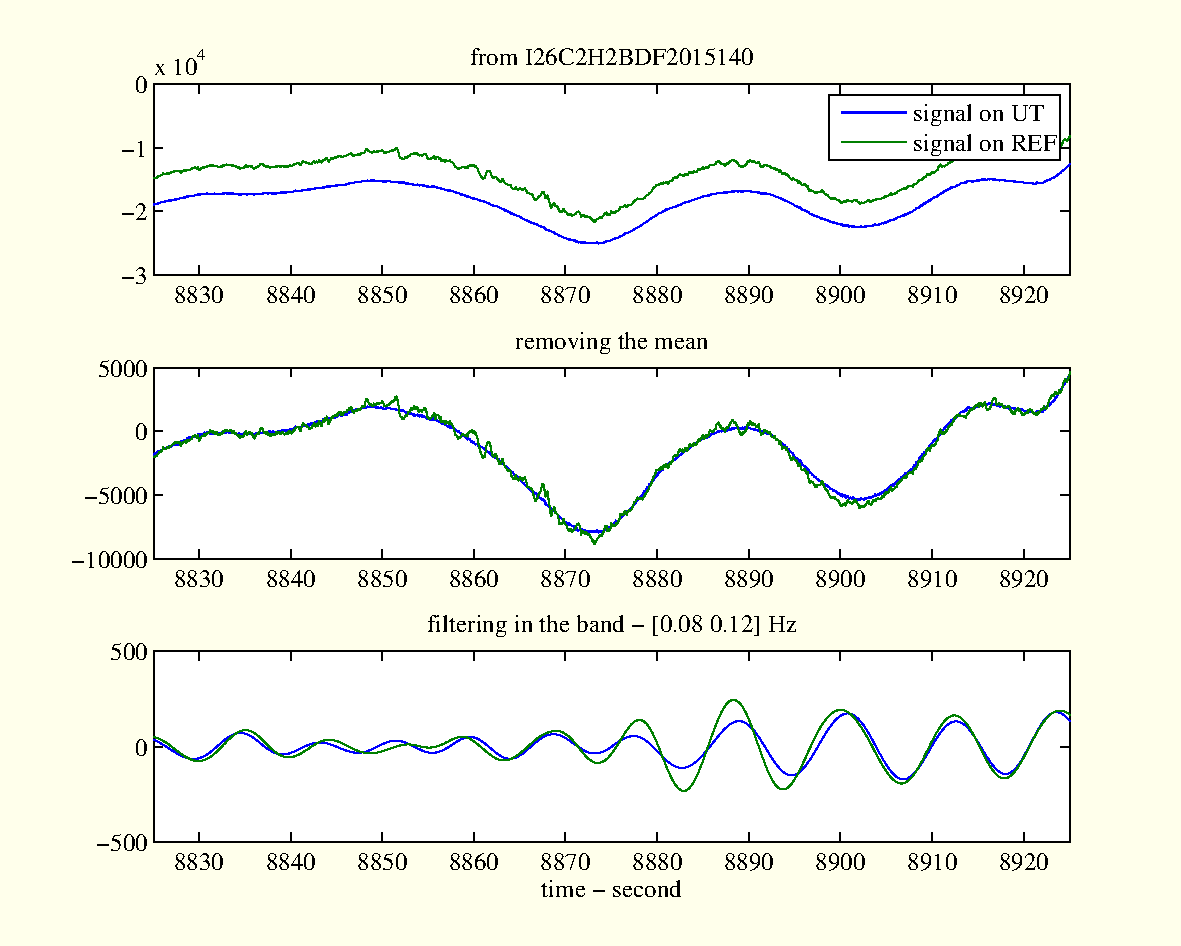
\includegraphics[scale=0.5]{signalsanomaly.pdf}
%\end{minipage}
%\begin{minipage}[c]{8cm}
%              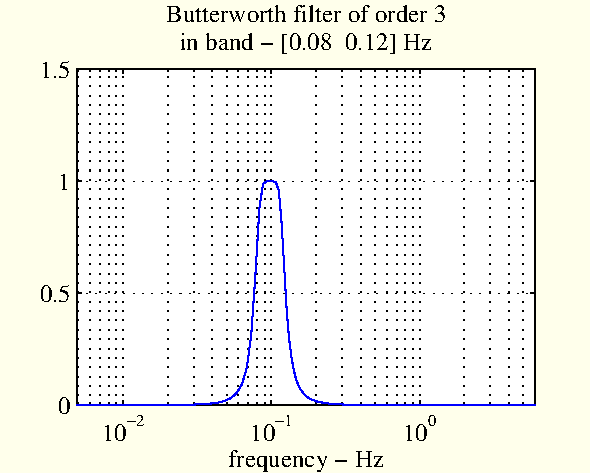
\includegraphics[scale=0.5]{filteranomaly.pdf}    
%
%\end{minipage}
%\centering
%\caption{Filtered signals}
%\label{fig:filteredsignals}
%\end{figure}
%


\clearpage
%============================================
%============================================
\section{Introduction}
%============================================
The noise reduction system (NSR) commonly used in front of the infrasonic sensors in the IMS stations is based on the property that the wind noise appears as spatially uncorrelated at the air inlets of the NRS. Therefore by summation, the SNR is improved in the ratio of the number of inlets. 

Unfortunately this gain is reduced in low frequencies as it has been observed by Alcoverro and al. \cite{alcoverro:2005}. This effect is characterized by the parameter $\zeta=v/f$ where $v$ denotes the wind velocity and $f$ the frequency. $\zeta$ can be interpreted as a ``wavelength'' and must be compared to the inlet inter-distances. If $\zeta$ is of the same order of magnitude of the inter distances, spatial coherence increases. It is not a good news, at first because the noise reduction  is lower. Another drawback occurs when we want to calibrate the sensor by using a second sensor without NRS. In this case the levels of the coherent part will be different and we have no way to identify it.

As a quantitative illustration for wind velocity above $5$ m/s, measurement is no more possible. But for velocity around $1$ m/s and for frequency under $0.01$ Hz, $\zeta>100$ m and the wind is seen as coherent by the full NSR. In the middle range for velocity around $1$ m/s and frequency around $0.1$ Hz, $\zeta\approx 10$ m and a part of the wind noise is seen as coherent just because the NRS. That can induce artefact in the {\it in-situ} calibration because the coherence level close to 1 does not guaranty that the system to solve is well determined.


This article proposes a model for the spatial coherency, as it observed in \cite{alcoverro:2005} and presents simulated and experimental results. This model is similar to the model proposed in \cite{nouvellet_itwb:2013} which is derived from the pioneer approach of Mack and Flinn \cite{mack_flinn:1971}.

%============================================
%============================================
\section{Model for wind turbulences}
Wind turbulence is a very complex air movement. Here we assume that it can be described (as a gray box) by a stationary random  process whose coherence matrix depends on the distance between two spatial locations. At first we just summarize useful definitions of stationary $M$-ary process.

%============================================
\subsection{Stationary $M$-ary process}
An $M$-ary process $x(t)=\begin{bmatrix}
x_{1}(t)&\ldots&x_{m}(t)&\ldots&x_{M}(t)
\end{bmatrix}^{T}$ is associated to a spatial-time description. More specifically, $t$ denotes the time and $m$ an index associated with the 3D spatial locations, usually related to a sensor array.  Therefore we have to consider spatial and temporal properties. For example, an $M$-ary process could be:
\begin{itemize}
 \item
temporally white, meaning that $\esp{x_m(t)x_m(t')}=0$ for $t\neq t'$,
\item
spatially white, meaning that $\esp{x_m(t)x_{m'}(t)}=0$ for $m\neq m'$.
\end{itemize} 
There is no relationship between these two notions. In the general case $\esp{x_m(t)x_{m'}(t')}$ does depend on $(m,m',t,t')$. Temporal stationarity refers to the property that the statistics do depend on $(t-t')$. Spatial ''stationarity'' is a littlebit more complicate because of the 3D coordinates. In some simple cases $\esp{x_m(t)x_{m'}(t')}$ could depend only on the distance between the 2 points indexed by $m,m'$. A particular case is when $\esp{x_m(t)x_{m'}(t')}=0$ for $m\neq m'$ which is called spatially white.

%============================================
\subsubsection{Spectral description}
When the process is a wide sense stationary (WSS) process  a spectral representation can be associated to the covariances. A zero-mean WSS  process is defined by the property that the covariance matrix $R(h)=\esp{x(t+h)x^{H}(t)}$ does not depend on $t$. It is also characterized by the spectral matrix which is the Fourier transform of the covariance matrix sequence:
\begin{eqnarray}
 \Gamma(f) = \int e^{-2j\pi fh}R(h)dh
\end{eqnarray}
where $\Gamma(f)$ is a square matrix of size $M$.

The most fundamental property says that, for any value of the frequency $f$, the spectral matrix is a non-negative matrix. Moreover if $x(t)$ is real, $\Gamma(f)=\Gamma(-f)$.

If the spectral matrix is of rank 1, the process is said spatially coherent. If the spectral matrix is diagonal we say that the process is spatially white. If the spectral matrix is rank deficient we say that the process is partially-coherent. A process whose spectral matrix $\Gamma(f)=\sigma^{2}I_{M}$ is both spatially and temporally  white, because $\Gamma(f)$ does not depend on $f$.

It is also common to consider the function
\begin{eqnarray}
\label{eq:correlationcoherence}
 C_{km}(f)
 &=&\frac{\Gamma_{km}(f)}{\sqrt{\Gamma_{kk}(f)\Gamma_{mm}(f)}}
\end{eqnarray}
where it is assumed that $\Gamma_{kk}(f)\Gamma_{mm}(f)\neq 0$. We can also use the matricial notation
\begin{eqnarray}
 \label{eq:def-generalMSC}
  C(f) = P^{-1}(f)  \Gamma(f) P^{-1}(f)
\end{eqnarray}
or
\begin{eqnarray}
 \label{eq:reverse-def-generalMSC}
  \Gamma(f) = P(f) C(f) P(f)
\end{eqnarray}
where
\begin{eqnarray}
  \label{eq:spectral-content}
 P(f) =   \begin{bmatrix}
  \Gamma_{11}^{1/2}(f)&0&\cdots&0
  \\
  0&\Gamma_{22}^{1/2}(f)&\cdots&0
  \\
  \vdots
  \\
  0&\cdots&0&\Gamma_{MM}^{1/2}(f)
  \end{bmatrix}
\end{eqnarray}
The $M$-ary matrix
\begin{eqnarray}
 \label{eq:coherence-matrix}
 C(f)=\begin{bmatrix}
1&C_{12}(f)&\ldots\\
C_{21}(f)&1& \ldots\\
\vdots\\
\ldots&\ldots&C_{M,M-1}(f)&1
\end{bmatrix}
\end{eqnarray}
is called the coherence matrix. The  function 
\begin{eqnarray}
 \label{eq:def-coherence-function}
 \MSC_{km}(f)=|C_{km}(f)|^{2}
\end{eqnarray}
is called the magnitude square coherence, in short MSC, between $x_{k}(t)$ and $x_{m}(t)$. 
It is easy to show that $\MSC_{km}(f)\leq 1$ and
\begin{eqnarray}
 \label{eq:rhomlfeq1}
 \MSC_{km}(f)=1,\quad \forall f
\end{eqnarray}
if and only if $x_{k}(t)$ and $x_{m}(t)$ are related by a linear filter. When $\MSC_{km}(f)=1$ for all pairs $(k,m)$ the spectral matrix is of rank $1$, hence 
\begin{eqnarray}
C(f)={\mathds 1}_M{\mathds 1}_M^T
\end{eqnarray}
and the process is fully coherent. 
%================================================================= 
\subsubsection{WSS filtering}
A fundamental property concerns the filtering. Let us consider an $M$-ary zero-mean WSS process $x(t)$ with the spectral matrix $\Gamma_x(f)$. Let $y(t)$ the $N$-ary process on the output of a multiple input multiple output (MIMO) filter whose frequency response is the matrix  $K(f)$ of size $N$ by $M$. Then $y(t)$ is a WSS process with zero-mean and whose the spectral matrix writes:
\begin{eqnarray}
 \label{eq:filteringMIMO}
 \Gamma_y(f)&=&K(f)\Gamma_x(f)K^H(f)
\end{eqnarray}
%================================================================
%================================================================
\subsection{Wind noise model}
%================================================================
Wind turbulence is a very complex air movement. Here we assume that it can be described by a stationary random  process whose coherence matrix as the following entry form \cite{nouvellet_itwb:2013}:
\begin{eqnarray}
\label{eq:sm-general-random}
C_{km}(f) = \int \exp(-2j\pi f (r_k-r_m)^T k ) \,p_K(k)dk
\end{eqnarray}
where $f$ is the frequency, $r_k$ and $r_m$ are any two 3D locations and $k$ the slownwess vector. $p_K(k)$ is a probability distribution in $\mathds{R}^{3}$ meaning that the slownwess vector is considered to be random.
Let assume at first that $k$ is deterministic, that writes $p_{\Delta}(u)du=\delta_{0}(du)$. Hence expression  \eqref{eq:sm-general-random} can be written:
\begin{eqnarray*}
C_{km}(f) = e^{-2j\pi f(r_k-r_m)^Tk_0}
\end{eqnarray*}
That means that the displacement is a plane wave. It is worth to notice that the matrix $C$ can be written:
\begin{eqnarray*}
C(f) = E(f)E^{H}(f), 
\quad\mathrm{with}\quad
E(f) = \begin{bmatrix}
e^{-2j\pi r_{1}^{T} k_0}&\ldots&e^{-2j\pi r_{M}^{T}k_0}
\end{bmatrix}^{T}
\end{eqnarray*}
Hence the multivariate process is fully coherent.

The model, derived from the pioneer work by Mack and Flinn \cite{mack_flinn:1971} for the loss of coherence, considers that the azimuth $a$, the elevation $e$ and velocity $v$ are random variables. More specifically, we assume that the 3D vector $\mu=(a,e,v)$ writes:
\begin{equation}
 \label{eq:randomnesswn}
 \mu=\mu_{0}+\nu
\end{equation} 
where $\mu_{0}=(a_{0},e_{0},v_{0})$ is a deterministic part and $\nu$ a zero-mean Gaussian random vector of dimension 3, whose covariance is denoted $\Sigma_{\mu}$. It is shown in the appendix that:
\begin{eqnarray}
\label{eq:Cfr1r2Gaussian}
C_{m,\ell}(f)=
\underbrace{e^{-2j\pi f(r_{m}-r_{\ell})^{T}k_{0}}}_{\text{pure delay}}
 \underbrace{e^{-2\pi^{2}(f/v_0)^{2}(r_{m}-r_{\ell})^{T}
                 \tilde \Sigma_{k}(r_{m}-r_{\ell})}}_{\text{coherence effect}}
 \end{eqnarray}
where $\tilde \Sigma_{k}$ is given by \eqref{eq:aec2theta}. We let $\zeta=v_0/f$ that appears as a ``wavelength''. Using the MSC definition \eqref{eq:def-coherence-function}  we derive the following expression:
\begin{eqnarray}
\label{eq:MSCwind}
\MSC_{km}(f)=
e^{-4\pi^{2}(r_{m}-r_{\ell})^{T}
                 \tilde \Sigma_{k}(r_{m}-r_{\ell})/\zeta^{2}}
 \end{eqnarray}

The same parameter $\zeta$ has been proposed by Alcoverro and al. in \cite{alcoverro:2005} to characterize the coherence of the wind disturbances for closely located sensors. The expression \eqref{eq:MSCwind} has a clear meaning: the coherence  between any two spatial locations decreases when the distance between them is large compared to the ''wavelength'' $\zeta$. 

It follows that when $\zeta$ is low, i.e. low wind velocity and/or high frequency, the wind signals on the different air inlets are almost uncorrelated hence $M$ works as a reduction factor. On the other hand when $\zeta$ is high, i.e. high wind velocity and/or low frequency, the wind signals on the different air inlets are strongly correlated hence that allows good conditions to estimate the ratio between the sensor responses. In the mid-range, it appears that the common signal is present with two different amplitudes on the two sensors inducing a ratio different from $1$. Simulation below gives an illustration of that.




%============================================
\subsection{Coherence level as a function of $v/d$}

To show that our model is in good agreement with the experimental results reported in  \cite{alcoverro:2005} we  consider the following simulation: we choose $M$ random locations in such a way we obtain several different inter-distances. Using the formula \eqref{eq:Cfr1r2Gaussian} we compute for each pair of locations the frequency $f_{c}$ associated with the coherence level of $0.5$. This value has been chosen in  \cite{alcoverro:2005} to define a cut-off for the MSC. We also compute the ratio $v/d$ where $d$ is the distance between the two locations. Finally the coordinate couples $(v/d,f_{c})$ are reported figure \ref{fig:f05asvond}. The obtained cloud shape figure is very similar to the observation values reported in
figure 5 of \cite{alcoverro:2005}. It is worth to notice that the frequency $f_{c}$ does not depend only on the distance. The reason is the coherence formula depends on the quadratic form $(r_m-r_k)^{T}\tilde \Sigma_{k}(r_m-r_k)$ and therefore on the angle between $(r_m-r_k)$ and the  eigenvectors of the matrix  $\tilde \Sigma_{k}$. This quadratic form reduces to the euclidian distance if $\tilde \Sigma_{k}\propto I_{3}$. 
 \figscale{f05asvond.pdf}{Frequency $f_c$ associated with the MSC level $0.5$ as a function of $v/d$. }{fig:f05asvond}{0.8}


 \newpage
%======================================================
%======================================================
 \section{Application to the {\it in-situ} calibration method}
%======================================================
%======================================================
 %\subsubsection{Coherence with/without NRS}
%======================================================



	We consider a sensor with its NRS. This sensor is called sensor under test (SUT). We also consider an other sensor with no NRS, representing the reference sensor (Sref). The NRS consists  of $M=96$ air identical inlets located at the ends of pipes. The scheme is reported on the figure \ref{fig:bigschema}. Thanks to the  Gabrielson's study \cite{gabrielson:2011}, the transfer function $U(f)$ between any inlet and the cavity center of the NRS can be performed as a function of the geometrical structure of the NRS.
% and the transfer function $H(f)$ associated to the reference sensor can be performed. 
%Calculation algorithm for the reference sensor gives $H(f)\approx 1$, hence the ratio $G(f)/H(f)\approx G(f)$ in the full frequency band.

\figscale{bigschema.pdf}{$S_{x}(f)$ spectral matrix de dimension $(M+1)$, $S_{y}(f)$ spectral matrix de dimension $2$, $S_{z}(f)$ spectral matrix de dimension $2$}{fig:bigschema}{0.6}

The spectral matrix of the $(M+1)$-ary input signal writes:
\begin{eqnarray}
\label{eq:Sxf}
 S_x(f) = \gamma_{s}(f) \mathds{1}_{M+1}\mathds{1}_{M+1}^T+ \Gamma(f)
\end{eqnarray}
where $\gamma_{s}(f)$ is the spectral density of the coherent part, which is generally acoustic. By acoustic we mean that the wave has a velocity $c$ of the order of magnitude of $300$ m/s. Let us notice that the associated wavelength of this acoustic part is greater  than 75 meter for any frequencies below 4 Hz.

We assume that the spectral square matrix $\Gamma(f)$, whose size is $(M+1)$, is given by the expression \eqref{eq:reverse-def-generalMSC}  where $C(f)$ entries are given by \eqref{eq:Cfr1r2Gaussian} and 
\begin{eqnarray}
  \label{eq:spectral-content}
 P(f) =   \begin{bmatrix}
  \gamma_{u}^{1/2}(f)&0&\cdots&&0&
  \\
  0&\gamma_{u}^{1/2}(f)&\cdots&&0&
  \\
  \vdots
  \\
  0&\cdots&0&\gamma_{u}^{1/2}(f)&0
  \\
  0&\cdots&&0&\gamma_{r}^{1/2}(f)
  \end{bmatrix}
\end{eqnarray}
Here it is assumed that the noise has the same level $\gamma_{u}(f)$ on all NRS inlets but is different on the reference sensor denoted $\gamma_{r}(f)$.

It follows that the $2\times 2$ spectral matrix associated to the signals at the inputs of the two sensors writes:
\begin{eqnarray}
\label{eq:Syf}
 S_y(f) = K(f) S_x(f) K^H(f)
 \end{eqnarray}
where
\begin{eqnarray*}
K(f)&=&
\begin{bmatrix}
U_{1}^*(f)&\ldots&U_{M}^*(f)&0
\\
0&\ldots&0&1
\end{bmatrix}
\end{eqnarray*}
where we assume that the transfer function of the pipe of the reference sensor is $1$. 

In the following we assume that $U_{1}(f)=\cdots= U_{M}(f)=U(f)$.

From \eqref{eq:Syf} we derive that:
\begin{eqnarray*}
\label{eq:Syentries}
S_{y,11}(f)&=&
|U(f)|^2 \, (M^2\gamma_{s}(f) + \gamma_{u}(f) S_M(f))
\\
S_{y,22}(f)&=&(\gamma_{s}(f) +\gamma_{r}(f))
\\
S_{y,12}(f)&=&
U^{*}(f)\, (M\gamma_{s}(f)+\gamma_{u}^{1/2}(f)\gamma_{r}^{1/2}(f)s_M(f))
\\
S_{y,21}(f)&=&S_{y,12}^{*}(f)
\end{eqnarray*}
where
\begin{eqnarray*}
 S_M(f) =\sum_{k=1}^{M}\sum_{k'=1}^{M}C_{k,k'}
&\mathrm{and}&
 s_M(f) =\sum_{k=1}^{M}C_{k,M+1}
\end{eqnarray*}
Let us notice that for small values of $\zeta$, the $(M+1)$ entries are spatially uncorrelated hence $C$ is the identity leading to
$S_M(f)=M$ and $s_M(f) =0$.

We denote 
\begin{eqnarray*}
S_{z}(f)&=&
\begin{bmatrix}
S_{UU}(f)&S_{UR}(f)
\\
S_{RU}(f)&S_{RR}(f)
\end{bmatrix}
\end{eqnarray*}
with
\begin{eqnarray}
\label{eq:Syentries}
S_{UU}(f)&=& |G_{u}(f)|^2 \,|U(f)|^2 \, (M^2 \gamma_{s}(f)+ \gamma_{u}(f) S_M(f))
\\
S_{RR}(f)&=&|G_{r}(f)|^2 (\gamma_{s}(f)+\gamma_{r}(f))
\\
S_{UR}(f)&=& G_{u}(f)G_{r}^{*}(f)U^{*}(f)\, 
   (M\gamma_{s}(f)+\gamma_{u}^{1/2}(f)\gamma_{r}^{1/2}(f)s_M(f))
\\
S_{RU}(f)&=&S_{UR}^{*}(f)
\end{eqnarray}
Let us remark that a perfect NRS would have $U(f)=1/M$ for all frequencies. Unfortunately that is not satisfied for high frequency values. Indeed it is known that the NRS presents a resonance above $2$ Hz.

At first  if we consider that $U(f)=1/M$, $S_M(f)=M$ and $s_{M}(f)=0$ then we obtain
\begin{eqnarray}
\label{eq:Syentries-idealcase}
S_{UU}(f)&=& |G_{u}(f)|^2  (\gamma_{s}(f)+ \gamma_{u}(f) /M)
\\
S_{RR}(f)&=&|G_{r}(f)|^2 (\gamma_{s}(f)+\gamma_{r}(f))
\\
S_{UR}(f)&=& G_{u}(f)G_{r}^{*}(f) \gamma_{s}(f)
\\
S_{RU}(f)&=&S_{UR}^{*}(f)
\end{eqnarray}
We recognize the classical expression which is the base of the {\it in-situ} calibration. We see also that the noise level is divided by $M$ which is what we expect using an NRS. Unfortunately, since  this ratio $\gamma_{u}(f)/\gamma_{r}(f)$ is unknown, the system is underdetermined. One way to circumvent  this problem is to consider that the wind noises are very close to zero. Indeed if $\gamma_{u}(f)=\gamma_{r}(f)=0$
\begin{eqnarray*}
 G_{u}(f) &=& \frac{S_{UU}(f)}{S_{RU}(f)}\, G_{r}(f)
\end{eqnarray*}


To test the zero-noise it is well-known that the MSC can be used but we have to keep in mind that the MSC equal 1 does not mean that the ratio between the sensor response is 1. It only means that the ratio is a transfer function as for example a pure number. It is the reason why the ratio presents a dip as we see below.

%==================================================================
\subsubsection{MSC}
%==================================================================
In this section we show that the MSC could be very close to 1 and the sensor frequency response ratio is not equal to 1. The MSC successively writes:
\begin{eqnarray}
\label{eq:RsuponM}
 \MSC(f) &=& \frac{|S_{UR}(f)|^2}{S_{UU}(f)S_{RR}(f)} \nonumber
 \\
 &=& \frac{|M\gamma_{s}(f)+\gamma_{u}^{1/2}(f)\gamma_{r}^{1/2}(f)s_M(f))|^2}
    {(M^2 \gamma_{s}(f)+ \gamma_{u}(f) S_M(f))(\gamma_{s}(f)+\gamma_{r}(f))}
\end{eqnarray}
We let $\rho_{i}(f)=\gamma_{i}(f)/\gamma_{s}(f)$. Then
\begin{eqnarray}
\label{eq:RsuponM-rho}
 \MSC(f) 
 &=& \frac{|M+\rho_{u}^{1/2}(f)\rho_{r}^{1/2}(f)s_M(f))|^2}
    {(M^2 + \rho_{u}(f) S_M(f))(1+\rho_{r}(f))}
\end{eqnarray}
It follows:
\begin{itemize}
 \item
For high frequencies $s_M(f)\approx 0$ and $S_M(f)\approx M$, hence 
\begin{eqnarray}
\label{eq:MSCHF}
 \MSC(f) 
 \approx \frac{1}{(1+\rho_{u}(f)/M)(1+\rho_{r}(f))}
\end{eqnarray}

 \item
For very low frequencies $s_M(f)= M$ and $S_M(f)= M^2$, hence:
\begin{eqnarray}
\label{eq:MSCBF}
 \MSC(f) = \frac{(1+\sqrt{\rho_{u}(f)\rho_{r}(f)})^{2}}{(1+\rho_{u}(f))(1+\rho_{r}(f))}
\end{eqnarray}
	the MSC could be close to $1$ even if $\rho_{u}(f)$ and $\rho_{r}(f)$ are different of 0.
 \item
For mid-range, $s_M(f)\approx \lambda_1 M$ and $S_M(f)\approx \lambda_2 M^{2}$, hence 
\begin{eqnarray}
\label{eq:MSCMidF}
 \MSC(f) \approx 
    \frac{(1+\lambda_{1}\sqrt{\rho_{u}(f)\rho_{r}(f)})^{2}}
           {(1+\lambda_{2} \rho_{u}(f))(1+\rho_{r}(f))}
\end{eqnarray}
If $\lambda_{1}$ and $\lambda_{2}$ are close to $1$, the MSC could be close to $1$ even with $\rho_{i}(f)\neq 0$.
\end{itemize}
In conclusion $\MSC(f)$ close to $1$ does not mean that  $\rho_{u}(f)$ and $\rho_{r}(f)$ are close to 0 and in this case the system is still underdetermined.



\newpage\clearpage
%==================================================================
\subsubsection{Frequency response ratio}
%==================================================================
Assuming that $U(f)=1/M$ for all frequencies, the frequency response ratio writes:
\begin{eqnarray*}
R(f)&=& 
\frac{S_{UU}(f)}{S_{UR}^{*}(f)}=\frac{ G_{u}(f)}{G_{r}(f)}\times
\frac{ 1+ \gamma_{u}(f) S_M(f)/M^{2} \gamma_{s}(f)}{
   1+\gamma_{u}^{1/2}(f)\gamma_{r}^{1/2}(f)s_M(f)/M \gamma_{s}(f)}
\end{eqnarray*}
if $\gamma_{u}(f) =\gamma_{r}(f) =1$, and $\gamma_{u}(f) =\rho\gamma_{s}(f)$:
\begin{eqnarray*}
R(f)&=& 
\frac{S_{UU}(f)}{S_{UR}^{*}(f)}=\frac{ G_{u}(f)/M}{G_{r}(f)}\times
\frac{M^{2}+ \rho S_M(f)}{M+ \rho s_M(f)}
\end{eqnarray*}
where the quantity $G_{u}(f)/M$ is provided by the Gabrielsson analysis and is very close to $1/M$, except above 2 Hz, due to the resonance effect. Numerical results are reported figure \ref{fig:GonH} for a given shape of $\rho(f)$.


  \figscale{GonH.pdf}{The top curve represents the spectral ratio $\rho(f)$. The two following curves report the magnitude and the phase of the ratio
   The blue parts of   corresponding to an MSC greater than $0.95$. For frequencies over $0.4$ Hz up to $4$ Hz and for low noise levels, the curves reproduce the response of the NRS. In particular on the high frequency part the curves are related to a known resonance effect. For frequencies under $0.08$ Hz and even for low values of $\SNR$, the coherence is very high, because the wind turbulences appear as spatially coherent. In the mid frequency range we can have simultaneously a high MSC and a ratio less than $1$.}{fig:GonH}{0.7}
  
%==================================================================
\newpage\clearpage
%==================================================================
\section{Numerical results in I26}
%==================================================================

\figscale{twospeeds}{Top figure: averaging of the wind speed on plain curve, standard deviation 
around the averaging in dotted curve. Markers indicate the two parts of interest. 
Bottom figure: curves associated to the two parts of interest. The shift between them has a ratio of about $4$ which is about the ratio of the speed means od the  two parts of interest.}{fig:twospeeds}{0.8}

\figscale{twospeedsbis}{see figure \ref{fig:twospeeds}}{fig:twospeedsbis}{0.7}

\figscale{twospeedster}{see figure \ref{fig:twospeeds}}{fig:twospeedster}{0.7}

